\section{B.a.-ba des mathématiques}

\begin{frame}[fragile=singleslide]
  \frametitle{Principes de base}
  \begin{itemize}
  \item Décrire des équations mathématiques requiert un «langage» spécial
    \begin{itemize}
    \item il faut informer {\LaTeX} que l'on passe à ce langage
    \item par le biais de modes mathématiques
    \end{itemize}
  \item Important d'utiliser un mode mathématique
    \begin{itemize}
    \item règles de typographie spéciales (constantes vs variables,
      disposition des équations, numérotation, etc.)
    \item espaces entre les symboles et autour des opérateurs gérées
      automatiquement
    \end{itemize}
  \item Vous voulez utiliser le paquetage \pkg{amsmath}
\begin{lstlisting}
\usepackage{amsmath}
\end{lstlisting}
    \begin{itemize}
    \item lire la documentation de ce paquetage pour connaître toutes
      ses fonctionnalités
    \end{itemize}
  \end{itemize}
\end{frame}

\begin{frame}[fragile]
  \frametitle{Modes mathématiques}
  \begin{enumerate}[<+->]
  \item «En ligne» directement dans le texte comme $(a + b)^2 = a^2 +
    2ab + b^2$ en plaçant l'équation entre \verb=$ $=
\begin{lstlisting}
«En ligne» directement dans le texte
comme $(a + b)^2 = a^2 + 2ab + b^2$
\end{lstlisting}
  \item «Hors paragraphe» séparé du texte principal comme
    \begin{equation*}
      \int_0^\infty f(x)\, dx = \sum_{i = 1}^n \alpha_i e^{x_i} f(x_i)
    \end{equation*}
    en utilisant divers types d'environnements
\begin{lstlisting}
«Hors paragraphe» séparé du texte principal comme
\begin{equation*}
  \int_0^\infty f(x)\, dx =
  \sum_{i = 1}^n \alpha_i e^{x_i} f(x_i)
\end{equation*}
\end{lstlisting}
  \end{enumerate}
\end{frame}

\begin{frame}[plain]
  \begin{conseil}
    Les équations, en ligne ou hors paragraphe, font partie intégrante
    de la phrase.

    \bigskip %
    Les règles de ponctuation usuelles s'appliquent donc aux
    équations.
  \end{conseil}

  \vspace{18pt}
  \fbox{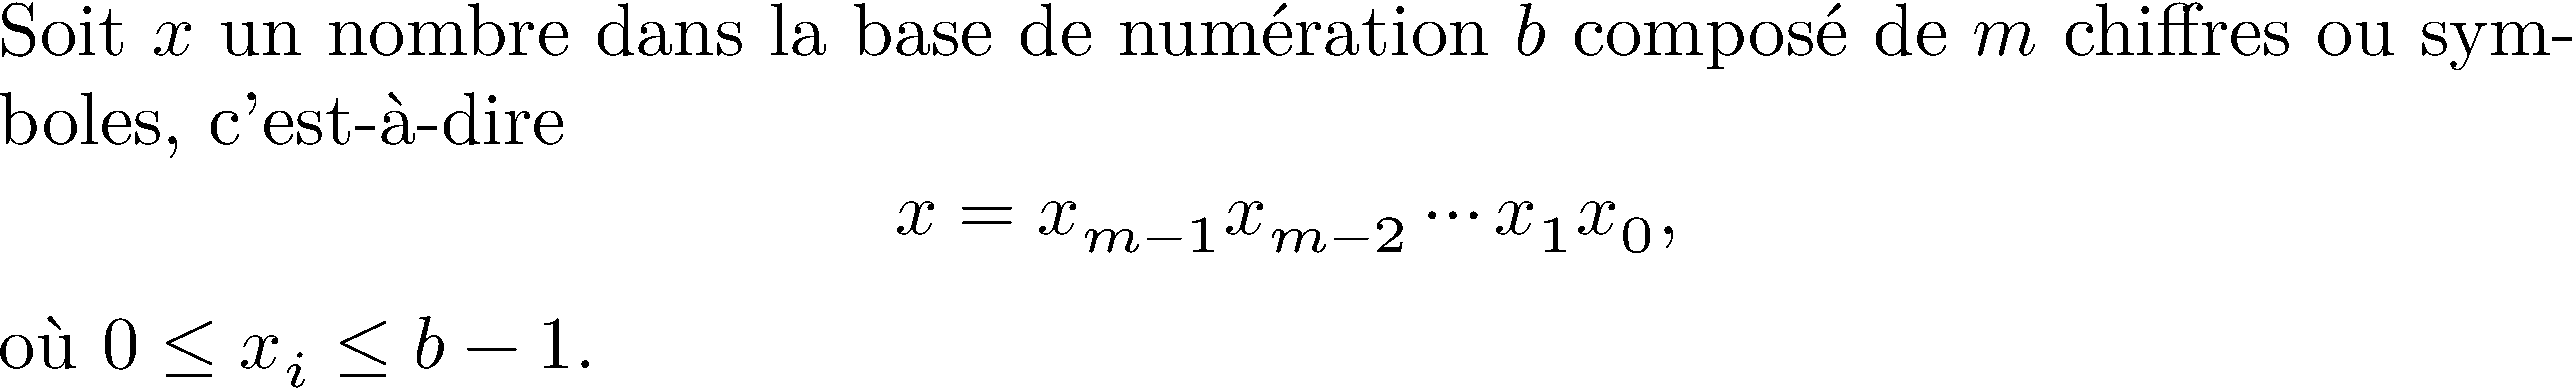
\includegraphics[width=0.95\linewidth]{ponctuation}}
\end{frame}

\begin{frame}[fragile]
  \frametitle{Quelques règles de base}
  \begin{itemize}
  \item En mode mathématique, {\TeX} respecte automatiquement la
    convention d'écrire les constantes en \rmfamily{romain} et les
    variables en \textit{italique}
    \begin{demo}
      \begin{texample}
\begin{lstlisting}
$z = 2a + 3y$
\end{lstlisting}
        \producing
        $z = 2a + 3y$
      \end{texample}
    \end{demo}
  \item Espace entre les éléments gérées automatiquement, peu importe
    le code source
    \begin{demo}
      \begin{texample}
\begin{lstlisting}
$z=2 a+3 y$
\end{lstlisting}
        \producing
        $z=2 a+3 y$
      \end{texample}
    \end{demo}
  \end{itemize}
\end{frame}

\begin{frame}[fragile]
  \frametitle{Quelques règles de base (suite)}
  \begin{itemize}
  \item \alert{Ne pas} utiliser le mode mathématique pour obtenir du
    texte en italique!
    \begin{demo}
      \begin{texample}
\begin{lstlisting}
\emph{xyz}
\end{lstlisting}
        \producing
        \rmfamily\emph{xyz}
      \end{texample}
      \begin{texample}
\begin{lstlisting}
$xyz$
\end{lstlisting}
        \producing
        $xyz$
      \end{texample}
    \end{demo}
  \item Utiliser la commande \verb=\text{}= de \pkg{amsmath} pour
    obtenir du texte à l'intérieur du mode mathématique
    \begin{demo}
      \begin{texample}
\begin{lstlisting}
$x = 0 \text{ si } y < 2$
\end{lstlisting}
        \producing
        $x = 0 \text{ si } y < 2$
      \end{texample}
    \end{demo}
  \end{itemize}
\end{frame}

\begin{frame}[fragile]
  \frametitle{Avant-goût}

  Pouvez-vous interpréter ce code?
\begin{lstlisting}
\begin{displaymath}
  \Gamma(\alpha) =
  \sum_{j = 0}^\infty \int_j^{j + 1}
    x^{\alpha - 1} e^{-x}\, dx
\end{displaymath}
\end{lstlisting}
  \vspace{18pt}
  \pause

  Fort probablement!
  \begin{displaymath}
    \Gamma(\alpha) =
    \sum_{j = 0}^\infty \int_j^{j + 1} x^{\alpha - 1} e^{-x}\, dx
  \end{displaymath}
\end{frame}

%%% Local Variables:
%%% mode: latex
%%% TeX-engine: xetex
%%% TeX-master: "formation-latex-ul-diapos"
%%% End:
